\graphicspath{{content/2_design/figures/}}
\section{Under-Voltage Protection}

\subsection{Configuration}

In order to protect the circuit from drawing too much current when the battery voltage is low, under-voltage protection will be employed.
A schmitt trigger will be used to detect when the battery voltage crosses over a specific threshold range. If the voltage
drops lower than a specified valued, the circuit will remove power from the two motors using a high-side PMOS switch. As soon as
the voltage rises above a slightly higher but specified value, the circuit will turn on power to the motors again.

The schmitt trigger will be non-inverting and will use a fixed voltage on the negative terminal as comparator reference.
This fixed voltage will be supplied via $\SI{5}{V}$ and will be divided down using two resistors. Its output will then pass through
an NMOS-PMOS combination to ultimately act as a high-side switch for the two motors.

\begin{figure}[!htb]
  \centering
  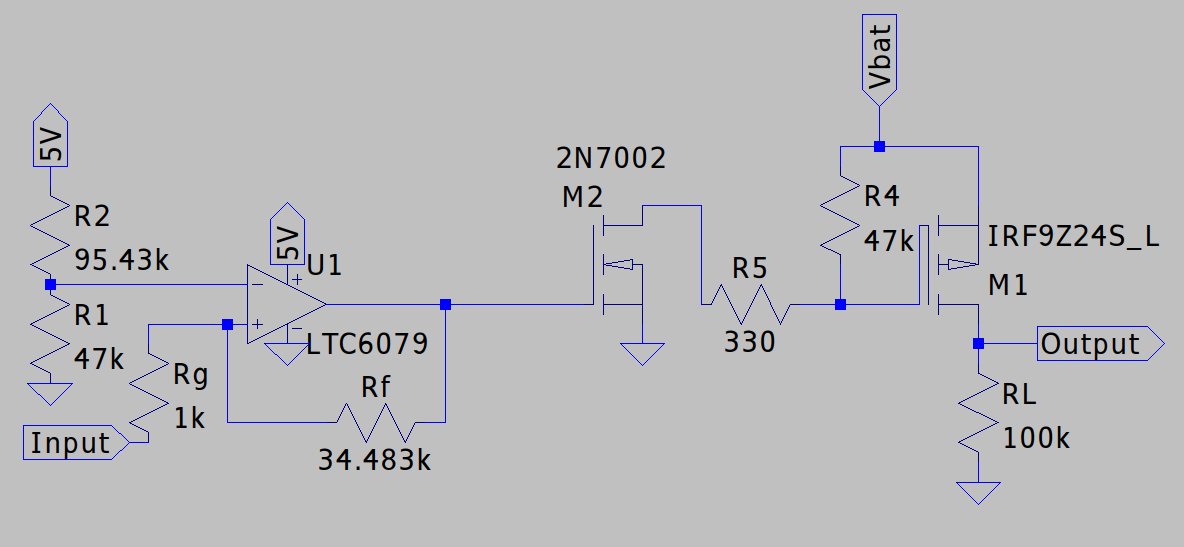
\includegraphics[width=0.6\textwidth]{underVoltageProtection_circuitDiagram}
  \caption{Under-Voltage Protection Circuit Diagram}
  \label{fig:underVoltageProtection_circuitDiagram}
\end{figure}

\subsection{Input Range}

The input to the circuit will be the output of the battery reader voltage with a range from 0.1 to 3.3 V. The battery voltage is not used directly,
as a fixed voltage is needed as a reference for the schmitt trigger. Since only 3.3 V or 5 V are available (the battery voltage is constantly changing),
the crossover point can be maximum 5 V. The choice of using the battery reader voltage also has the benefit of a wider range for the schmitt trigger.
The PMOS should therefore switch on when $V_i > 1.45 \times \SI{6}{V} - 7.17 = \SI{1.555}{V}$ and switch off when $V_i < \SI{1.7}{V}$.

\subsection{Design}

First, a KCL can be done at the positive terminal to show that $V_+ = \frac{R_f}{R_f + R_g} V_i + \frac{R_g}{R_f + R_g} V_o$.
When this voltage is greater than the voltage at the negative terminal, $V_-$ or $V_{ref}$, then the op-amp will saturate at the positive rail.
Conversely, the op-amp will saturate if $V_+ < V_{ref}$.

It can further be calculated that $V_i = V_+ + \frac{R_g}{R_f}(V_+ - V_o)$. If $V_{o(sat,high)} = \SI{5}{V}$ and $V_{o(sat,low)} = \SI{0}{V}$, resistor values can then calculated:

\begin{itemize}
    \item The lower threshold voltage is given as $\SI{3}{V}$. This gives the equation at which the output starts to saturate at the negative rail when already saturated at the positive rail.
          For this case, $\SI{1.555}{V} = V_{ref} + \frac{R_g}{R_f} (V_{ref} - \SI{5}{V})$.
    \item Similarly, the upper threshold voltage gives $\SI{1.7}{V} = V_{ref} + \frac{R_g}{R_f} V_{ref}$.
    \item Solving the above equations simultaneously yields $V_{ref} = \SI{1.652}{V}$ and $\frac{R_g}{R_f} = 0.029$.
    \item For $V_{ref}$, choose $R_1= \SI{47}{\kilo\ohm}$ therefore $R_2 = \SI{95.252}{\kilo\ohm}$. Choose $R_2 = \SI{82}{\kilo\ohm} + \SI{47}{\kilo\ohm}$pot.
    \item For $R_f$ and $R_g$, $\frac{R_g}{R_f} = 0.029$. Choose $R_g = \SI{1}{\kilo\ohm}$ and $R_f = \SI{34.483}{\kilo\ohm}$, with $R_f = \SI{27}{\kilo\ohm} + \SI{10}{\kilo\ohm}$pot.
\end{itemize}